\documentclass{article}%
\usepackage[T1]{fontenc}%
\usepackage[utf8]{inputenc}%
\usepackage{lmodern}%
\usepackage{textcomp}%
\usepackage{lastpage}%
\usepackage[head=40pt,margin=0.5in,bottom=0.6in]{geometry}%
\usepackage{graphicx}%
%
\title{\textbf{Isabel Coixet dirigirá su primera serie para HBO, "Foodie Love"}}%
\author{DPA}%
\date{07/03/2019}%
%
\begin{document}%
\normalsize%
\maketitle%
\textbf{URL: }%
http://www.eluniversal.com/entretenimiento/35001/isabel{-}coixet{-}dirigira{-}su{-}primera{-}serie{-}foodie{-}love{-}para{-}hbo\newline%
%
\textbf{Periodico: }%
EU, %
ID: %
35001, %
Seccion: %
entretenimiento\newline%
%
\textbf{Palabras Claves: }%
NO\_TIENE\newline%
%
\textbf{Derecho: }%
2.1%
, Otros Derechos: %
\newline%
%
\textbf{\textit{La cineasta española mezcla su pasión por las historias de amor y la gastronomía en su nuevo proyecto}}%
\newline%
\newline%
%
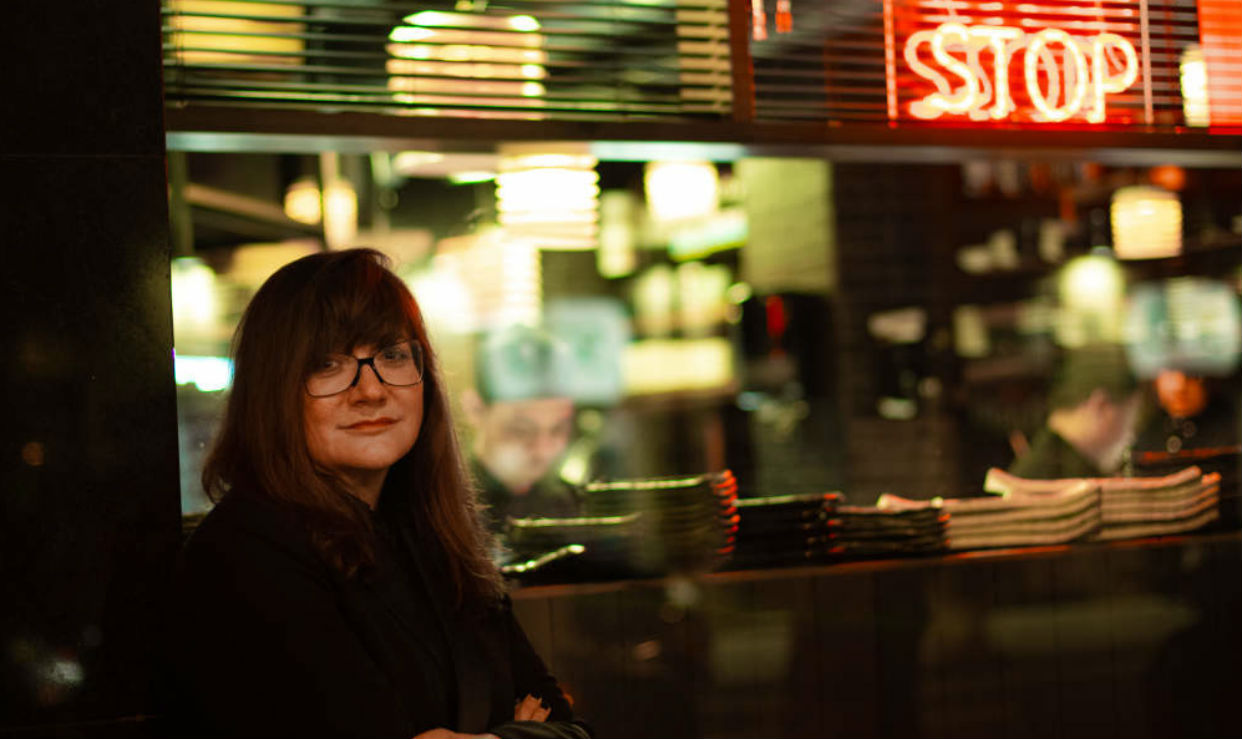
\includegraphics[width=300px]{EU_35001.jpg}%
\newline%
%
HBO da luz verde a la que será la primera serie de Isabel Coixet,%
\newline%
%
, cuyo rodaje arrancará este año.%
\newline%
%
La sinopsis oficial de la serie dice: "El algoritmo de una aplicación para encontrar pareja entre amantes de la gastronomía conecta a los protagonistas de Foodie Love, una chica y un chico que comienzan a conocerse con las dudas propias de quien conserva cicatrices de relaciones anteriores. A lo largo de varias citas tendrán que descubrir si coincidencias como su devoción por el yuzu japonés o su alergia común al postureo foodie son suficientes para construir los cimientos de una historia de amor duradera".%
\newline%
%
Coixet es la realizadora más aclamada de España. Cosecha un total de siete premios Goya y es responsable de grandes títulos como Mi vida sin mí (Seleccionada en el Festival de Berlín), La vida secreta de las palabras (Seleccionada en el Festival de Venecia), Mapa de los sonidos de Tokio (Seleccionada en el Festival de Cannes) o La librería, ganadora del Goya a la mejor película en 2018.%
\newline%
%
Para la directora, Foodie Love es "la fusión de dos de mis pasiones: las historias de amor y la comida {[}...{]} donde dos personajes se encuentran, se alejan y se reencuentran a través de un peculiar recorrido por cafés, bares, chiringuitos y restaurantes".%
\newline%
%
Coixet cataloga a sus protagonistas como "dos seres tímidos, fuertes, a ratos atormentados, a ratos despreocupados, que luchan por entenderse y entregarse el uno al otro".%
\newline%
%
Producida por Miss Wasabi Films, la serie "se nutre de todos los lugares en los que he estado, de todas las cosas que he probado. Y de muchas de las cosas que he vivido", reconoce la creadora.%
\newline%
%
\end{document}